\section{Performance Benchmarks}

We conducted several performance benchmarks to measure the throughput and scalability of our system. All these tests were performed on a LAN system called Lattice which has a network bandwidth of 1 Gbps. All nodes are Intel(R) Xeon(R) 2.4GHz 4 core duo machines with 16 GB of memory. We used Apache S4 0.6.0 version and Apache storm 0.9.2 version. Sample code used for all tests can be found here \cite{solutionCode}.


\subsection{Effect of message buffer size and thread pool}
For this experiment, we used a graph as shown in Figure \ref{ecgGraph} to process ECG signal data. The EventProducer reads a file containing over 7500000
 ECG records and pushes events with multiple threads. EventReceiver receives the ECG events, processes them and calculates heart rate interval periodically using Pan Tompkins algorithm \cite{kohler2002principles}. 

\begin{figure}[!t]
        \centering
        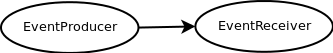
\includegraphics[width=2.0in]{ecgGraph.png}
        \caption{ECG Process Graph}
        \label{ecgGraph}
\end{figure}


We measured the throughput between two nodes for different thread pool and message buffer sizes to understand the effect of those parameters to throughput. As shown in figure \ref{throughputvar} throughput increases clearly with the message buffer size and increase with thread pool size for larger message buffer sizes. Therefore we can conclude both make a positive impact on the throughput.

\begin{figure}[!t]
        \centering
        \includegraphics[width=3.0in]{throughputvar.png}
        \caption{Throughput variation with the thread pool size and message buffer size.}
        \label{throughputvar}
\end{figure}

\subsection{Load balancing}

We used the same graph (Figure \ref{ecgGraph}) used in above experiment with 1,2 and 4 \textit{EventReciver} nodes with one \textit{EventSender} node for this experiment. Since 40 thread pool size and 40 message buffer size gives highest throughput, we used that values with our solution (named as Granules). Further we compared our system with Yahoo S4 \cite{neumeyer2010s4} and Twitter Storm \cite{toshniwal2014storm} with the same graph. Twitter Storm \cite{toshniwal2014storm} places tasks arbitrarily within the available nodes. Therefore we used 1 task for \textit{EventSender} and 1,2 and 4 tasks for \textit{EventReceivers} to place them in different nodes. This makes Twitter Storm \cite{toshniwal2014storm} execute only one thread to process data in each node. In order to compare this situation, we measured our system performance with 1 thread and 10 message buffer size as well.   

Figure \ref{throuput} shows the throughput of the systems. All systems keep initial throughput when increasing nodes. But our solution out performs all the other systems. Figure \ref{networkusage} shows the network bandwidth at each node (measured using atop linux command). For each framework sending node consumes same amount of network bandwidth since it sends all messages to other nodes. For receiving side each receiving node consumes corresponding portion of the bandwidth according to number of receiving nodes. For an example for 4 node configuration each receiving node consumes only one fourth of the sending node bandwidth. Compared to other systems our solution consumes all the available bandwidth. 

\begin{figure}[!t]
        \centering
        \includegraphics[width=3.0in]{throughput.png}
        \caption{Throughput comparison of S4, Storm and our solution.}
        \label{throuput}
\end{figure}

\begin{figure}[!t]
        \centering
        \includegraphics[width=3.0in]{network.png}
        \caption{Network usage at each node. For multiple receiving nodes it is the network utilization at a one node.}
        \label{networkusage}
\end{figure}


\subsection{Multistage Graph Processing}
We performed a multi-stage graph test for our system using the 3-level graph shown in Figure \ref{multigraph}. The data as well as the processing logic were obtained from the Grand Challenge problem at 8th ACM International Conference on Distributed Event Based Systems \cite{acm}. This project explores the possibility of using stream processing to process data generated in the smart grid domain. The data is generated by sensors attached to a device called “smart plug” which is plugged as an intermediate layer between a power outlet and the plug of a home appliance. The sensors capture various measures related to power consumption of each connected device and send these measurements continuously to a central processing system. Each household contains several of such smart plugs which will report the sensor readings once in every second. At the central processing system, these data should be processed in order to forecast the short time load and to generate load statistics for real time demand management. We implemented the first part of this project which predicts the load using a machine learning algorithm. This algorithm divides the events to fixed intervals called  time slices and uses average value of time slices to predict the average of feature time slices. We used the publicly available 500MB of data set to generate the events.

\begin{figure}[!t]
        \centering
        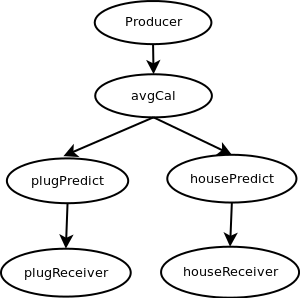
\includegraphics[width=2.0in]{multigraph.png}
        \caption{Multilevel Node Graph}
        \label{multigraph}
\end{figure}

As shown in Figure \ref{multigraph}, Producer node reads the data file and emits events to the \textit{avgCal} node which calculates the last time slice average and sends the same event to both \textit{plugPredict} and \textit{housePredict} processors. Both \textit{plugPredict} and \textit{housePredict} processors predict the next values and send events to receivers. The original problem only requires to send those prediction events in 30s intervals. But we used a prediction event for each messages to observe how the system works with high load. 

As in the earlier case, we conducted our experiments using one producer and incrementing the other processing nodes by 1, 2 and 4 times to measure the throughput increase at the producer. We ran each node in a separate machine so that our receiver configurations used 5, 10, 15 machines respectively. All nodes were configured to use both thread pool and message buffer size of 40. We measured the throughput, network bandwidth and the CPU load average at the producer to examine the scalability of the system. Since the one receiver unit throughput is greater than that of the Twitter Storm \cite{toshniwal2014storm} one node scenario, we only used our system for this experiment. As shown in Figure \ref{scalability} system scales up until it fully utilized the available network bandwidth.
 
\begin{figure*}[!t]
        \centering
        \subfloat[Throughput of the System]{\includegraphics[width=3.0in]{throughputs.png}}
        \hfil
        \subfloat[Network Usage (\%) at Sender]{\includegraphics[width=3.0in]{networkps.png}}
        \hfil
        \subfloat[Network Usage Bandwidth at Sender]{\includegraphics[width=3.0in]{networks.png}}
        \hfil
        \subfloat[CPU Load Average at Sender]{\includegraphics[width=3.0in]{loadaverages.png}}
        \caption{Performance of Multistage Graph processing.}
        \label{scalability}
\end{figure*}

\subsection{Scalability and Latency}
We analyze the scalability of our framework using cumulative throughput with a similar experiments found in research literature \cite{murray2013naiad} \cite{zaharia2013discretized}.  In this experiment a given set of nodes communicate directly with each other using TCP connections.  We used same message type (46 bytes in serialized format) used for earlier experiment. The given cumulative throughput is at the application level message rate omitting the TCP overhead and all communications are through the network. For all experiments we use 20 message buffer. Since each node is capable of sending and receiving 1Gbps of data, ideal throughput is same as number of nodes times 1Gbps. 

\begin{figure}[!t]
        \centering
        \includegraphics[width=3.0in]{allthroughput.png}
        \caption{All to All exchange Throughput}
        \label{allthroughput}
\end{figure}

As shown in Figure \ref{allthroughput} system linearly scales with the number of nodes.  Compared to Naiad (Figure 6(a) in cited paper) \cite{murray2013naiad} and Spark Streaming (Figure 4 in cited paper) \cite{zaharia2013discretized} we have achieved better performance (comparing the values given in those papers).  Figure \ref{alllatency} shows the mean message latency for all messages. We measured the message latency during the same experiment by sending the time stamp along with each message. Compared to Spark Streaming (Figure 4 in cited paper) \cite{zaharia2013discretized} we have achieved much lesser latency level. Naiad (Figure 6(b) in cited paper) \cite{murray2013naiad} reports very low latency for global barrier messages. However our latency corresponds to message latency for data messages. MillWheel (Section 8.1) \cite{akidau2013millwheel} has reported very low latency level compared to our results. Further it is worth note that the latency can be reduced by reducing the buffer size and hence reducing the throughput. We choose 20 message buffer since it gives better throughput as well as comparable low latency.

\begin{figure}[!t]
        \centering
        \includegraphics[width=3.0in]{alllatency.png}
        \caption{All to All exchange Latency}
        \label{alllatency}
\end{figure}


\subsection{Fault tolerance}
For this experiment we analyzed the resilience of the system in the presence of node failures. Initially we had a load balanced system where the event producer sends events to 8 receiving nodes. The producer produced messages at the rate of around 2500000 and each receiving node receive messages at a rate around 320000 ($\sim$ 2500000 / 8). Then we shutdown one process by one process within 1 minute interval. This increased the throughput of each receiving node. Figure \ref{rthroughput} shows the throughput received at the last node to shutdown with the time. As depicts in the Figure \ref{rthroughput} when a node fails system automatically removes the node from its configurations and route the messages to other nodes balancing load among existing ones.

\begin{figure}[!t]
        \centering
        \includegraphics[width=3.0in]{failure_throughput.png}
        \caption{Receiver throughput variation at the last node.}
        \label{rthroughput}
\end{figure}
